%% bare_conf.tex
%% V1.3
%% 2007/01/11
%% by Michael Shell
%% See:
%% http://www.michaelshell.org/
%% for current contact information.
%%
%% This is a skeleton file demonstrating the use of IEEEtran.cls
%% (requires IEEEtran.cls version 1.7 or later) with an IEEE conference paper.
%%
%% Support sites:
%% http://www.michaelshell.org/tex/ieeetran/
%% http://www.ctan.org/tex-archive/macros/latex/contrib/IEEEtran/
%% and
%% http://www.ieee.org/

%%*************************************************************************
%% Legal Notice:
%% This code is offered as-is without any warranty either expressed or
%% implied; without even the implied warranty of MERCHANTABILITY or
%% FITNESS FOR A PARTICULAR PURPOSE! 
%% User assumes all risk.
%% In no event shall IEEE or any contributor to this code be liable for
%% any damages or losses, including, but not limited to, incidental,
%% consequential, or any other damages, resulting from the use or misuse
%% of any information contained here.
%%
%% All comments are the opinions of their respective authors and are 
%% not necessarily endorsed by the IEEE.
%%
%% This work is distributed under the LaTeX Project Public License (LPPL)
%% ( http://www.latex-project.org/ ) version 1.3, and may be freely used,
%% distributed and modified. A copy of the LPPL, version 1.3, is included
%% in the base LaTeX documentation of all distributions of LaTeX released
%% 2003/12/01 or later.
%% Retain all contribution notices and credits.
%% ** Modified files should be clearly indicated as such, including  **
%% ** renaming them and changing author support contact information. **
%%
%% File list of work: IEEEtran.cls, IEEEtran_HOWTO.pdf, bare_adv.tex,
%%                    bare_conf.tex, bare_jrnl.tex, bare_jrnl_compsoc.tex
%%*************************************************************************

% *** Authors should verify (and, if needed, correct) their LaTeX system  ***
% *** with the testflow diagnostic prior to trusting their LaTeX platform ***
% *** with production work. IEEE's font choices can trigger bugs that do  ***
% *** not appear when using other class files.                            ***
% The testflow support page is at:
% http://www.michaelshell.org/tex/testflow/



% Note that the a4paper option is mainly intended so that authors in
% countries using A4 can easily print to A4 and see how their papers will
% look in print - the typesetting of the document will not typically be
% affected with changes in paper size (but the bottom and side margins will).
% Use the testflow package mentioned above to verify correct handling of
% both paper sizes by the user's LaTeX system.
%
% Also note that the "draftcls" or "draftclsnofoot", not "draft", option
% should be used if it is desired that the figures are to be displayed in
% draft mode.
%
\documentclass[conference]{IEEEtran}
% Add the compsoc option for Computer Society conferences.
%
% If IEEEtran.cls has not been installed into the LaTeX system files,
% manually specify the path to it like:
% \documentclass[conference]{../sty/IEEEtran}



% Some very useful LaTeX packages include:
% (uncomment the ones you want to load)


% *** MISC UTILITY PACKAGES ***
%
%\usepackage{ifpdf}
% Heiko Oberdiek's ifpdf.sty is very useful if you need conditional
% compilation based on whether the output is pdf or dvi.
% usage:
% \ifpdf
%   % pdf code
% \else
%   % dvi code
% \fi
% The latest version of ifpdf.sty can be obtained from:
% http://www.ctan.org/tex-archive/macros/latex/contrib/oberdiek/
% Also, note that IEEEtran.cls V1.7 and later provides a builtin
% \ifCLASSINFOpdf conditional that works the same way.
% When switching from latex to pdflatex and vice-versa, the compiler may
% have to be run twice to clear warning/error messages.






% *** CITATION PACKAGES ***
%
\usepackage{cite}
% cite.sty was written by Donald Arseneau
% V1.6 and later of IEEEtran pre-defines the format of the cite.sty package
% \cite{} output to follow that of IEEE. Loading the cite package will
% result in citation numbers being automatically sorted and properly
% "compressed/ranged". e.g., [1], [9], [2], [7], [5], [6] without using
% cite.sty will become [1], [2], [5]--[7], [9] using cite.sty. cite.sty's
% \cite will automatically add leading space, if needed. Use cite.sty's
% noadjust option (cite.sty V3.8 and later) if you want to turn this off.
% cite.sty is already installed on most LaTeX systems. Be sure and use
% version 4.0 (2003-05-27) and later if using hyperref.sty. cite.sty does
% not currently provide for hyperlinked citations.
% The latest version can be obtained at:
% http://www.ctan.org/tex-archive/macros/latex/contrib/cite/
% The documentation is contained in the cite.sty file itself.

%\usepackage{natbib}




% *** GRAPHICS RELATED PACKAGES ***
%
\usepackage[pdftex]{graphicx}
  % declare the path(s) where your graphic files are
\graphicspath{{C:/Kobus/Studies/MEM/Thesis/}}
  % and their extensions so you won't have to specify these with
  % every instance of \includegraphics
\DeclareGraphicsExtensions{.pdf,.jpeg,.png}

\ifCLASSINFOpdf
  % \usepackage[pdftex]{graphicx}
  % declare the path(s) where your graphic files are
  % \graphicspath{{../pdf/}{../jpeg/}}
  % and their extensions so you won't have to specify these with
  % every instance of \includegraphics
  % \DeclareGraphicsExtensions{.pdf,.jpeg,.png}
\else
  % or other class option (dvipsone, dvipdf, if not using dvips). graphicx
  % will default to the driver specified in the system graphics.cfg if no
  % driver is specified.
  % \usepackage[dvips]{graphicx}
  % declare the path(s) where your graphic files are
  % \graphicspath{{../eps/}}
  % and their extensions so you won't have to specify these with
  % every instance of \includegraphics
  % \DeclareGraphicsExtensions{.eps}
\fi
% graphicx was written by David Carlisle and Sebastian Rahtz. It is
% required if you want graphics, photos, etc. graphicx.sty is already
% installed on most LaTeX systems. The latest version and documentation can
% be obtained at: 
% http://www.ctan.org/tex-archive/macros/latex/required/graphics/
% Another good source of documentation is "Using Imported Graphics in
% LaTeX2e" by Keith Reckdahl which can be found as epslatex.ps or
% epslatex.pdf at: http://www.ctan.org/tex-archive/info/
%
% latex, and pdflatex in dvi mode, support graphics in encapsulated
% postscript (.eps) format. pdflatex in pdf mode supports graphics
% in .pdf, .jpeg, .png and .mps (metapost) formats. Users should ensure
% that all non-photo figures use a vector format (.eps, .pdf, .mps) and
% not a bitmapped formats (.jpeg, .png). IEEE frowns on bitmapped formats
% which can result in "jaggedy"/blurry rendering of lines and letters as
% well as large increases in file sizes.
%
% You can find documentation about the pdfTeX application at:
% http://www.tug.org/applications/pdftex





% *** MATH PACKAGES ***
%
%\usepackage[cmex10]{amsmath}
% A popular package from the American Mathematical Society that provides
% many useful and powerful commands for dealing with mathematics. If using
% it, be sure to load this package with the cmex10 option to ensure that
% only type 1 fonts will utilized at all point sizes. Without this option,
% it is possible that some math symbols, particularly those within
% footnotes, will be rendered in bitmap form which will result in a
% document that can not be IEEE Xplore compliant!
%
% Also, note that the amsmath package sets \interdisplaylinepenalty to 10000
% thus preventing page breaks from occurring within multiline equations. Use:
%\interdisplaylinepenalty=2500
% after loading amsmath to restore such page breaks as IEEEtran.cls normally
% does. amsmath.sty is already installed on most LaTeX systems. The latest
% version and documentation can be obtained at:
% http://www.ctan.org/tex-archive/macros/latex/required/amslatex/math/





% *** SPECIALIZED LIST PACKAGES ***
%
%\usepackage{algorithmic}
% algorithmic.sty was written by Peter Williams and Rogerio Brito.
% This package provides an algorithmic environment fo describing algorithms.
% You can use the algorithmic environment in-text or within a figure
% environment to provide for a floating algorithm. Do NOT use the algorithm
% floating environment provided by algorithm.sty (by the same authors) or
% algorithm2e.sty (by Christophe Fiorio) as IEEE does not use dedicated
% algorithm float types and packages that provide these will not provide
% correct IEEE style captions. The latest version and documentation of
% algorithmic.sty can be obtained at:
% http://www.ctan.org/tex-archive/macros/latex/contrib/algorithms/
% There is also a support site at:
% http://algorithms.berlios.de/index.html
% Also of interest may be the (relatively newer and more customizable)
% algorithmicx.sty package by Szasz Janos:
% http://www.ctan.org/tex-archive/macros/latex/contrib/algorithmicx/




% *** ALIGNMENT PACKAGES ***
%
%\usepackage{array}
% Frank Mittelbach's and David Carlisle's array.sty patches and improves
% the standard LaTeX2e array and tabular environments to provide better
% appearance and additional user controls. As the default LaTeX2e table
% generation code is lacking to the point of almost being broken with
% respect to the quality of the end results, all users are strongly
% advised to use an enhanced (at the very least that provided by array.sty)
% set of table tools. array.sty is already installed on most systems. The
% latest version and documentation can be obtained at:
% http://www.ctan.org/tex-archive/macros/latex/required/tools/


%\usepackage{mdwmath}
%\usepackage{mdwtab}
% Also highly recommended is Mark Wooding's extremely powerful MDW tools,
% especially mdwmath.sty and mdwtab.sty which are used to format equations
% and tables, respectively. The MDWtools set is already installed on most
% LaTeX systems. The lastest version and documentation is available at:
% http://www.ctan.org/tex-archive/macros/latex/contrib/mdwtools/


% IEEEtran contains the IEEEeqnarray family of commands that can be used to
% generate multiline equations as well as matrices, tables, etc., of high
% quality.


%\usepackage{eqparbox}
% Also of notable interest is Scott Pakin's eqparbox package for creating
% (automatically sized) equal width boxes - aka "natural width parboxes".
% Available at:
% http://www.ctan.org/tex-archive/macros/latex/contrib/eqparbox/





% *** SUBFIGURE PACKAGES ***
%\usepackage[tight,footnotesize]{subfigure}
% subfigure.sty was written by Steven Douglas Cochran. This package makes it
% easy to put subfigures in your figures. e.g., "Figure 1a and 1b". For IEEE
% work, it is a good idea to load it with the tight package option to reduce
% the amount of white space around the subfigures. subfigure.sty is already
% installed on most LaTeX systems. The latest version and documentation can
% be obtained at:
% http://www.ctan.org/tex-archive/obsolete/macros/latex/contrib/subfigure/
% subfigure.sty has been superceeded by subfig.sty.



%\usepackage[caption=false]{caption}
%\usepackage[font=footnotesize]{subfig}
% subfig.sty, also written by Steven Douglas Cochran, is the modern
% replacement for subfigure.sty. However, subfig.sty requires and
% automatically loads Axel Sommerfeldt's caption.sty which will override
% IEEEtran.cls handling of captions and this will result in nonIEEE style
% figure/table captions. To prevent this problem, be sure and preload
% caption.sty with its "caption=false" package option. This is will preserve
% IEEEtran.cls handing of captions. Version 1.3 (2005/06/28) and later 
% (recommended due to many improvements over 1.2) of subfig.sty supports
% the caption=false option directly:
%\usepackage[caption=false,font=footnotesize]{subfig}
%
% The latest version and documentation can be obtained at:
% http://www.ctan.org/tex-archive/macros/latex/contrib/subfig/
% The latest version and documentation of caption.sty can be obtained at:
% http://www.ctan.org/tex-archive/macros/latex/contrib/caption/




% *** FLOAT PACKAGES ***
%
%\usepackage{fixltx2e}
% fixltx2e, the successor to the earlier fix2col.sty, was written by
% Frank Mittelbach and David Carlisle. This package corrects a few problems
% in the LaTeX2e kernel, the most notable of which is that in current
% LaTeX2e releases, the ordering of single and double column floats is not
% guaranteed to be preserved. Thus, an unpatched LaTeX2e can allow a
% single column figure to be placed prior to an earlier double column
% figure. The latest version and documentation can be found at:
% http://www.ctan.org/tex-archive/macros/latex/base/



%\usepackage{stfloats}
% stfloats.sty was written by Sigitas Tolusis. This package gives LaTeX2e
% the ability to do double column floats at the bottom of the page as well
% as the top. (e.g., "\begin{figure*}[!b]" is not normally possible in
% LaTeX2e). It also provides a command:
%\fnbelowfloat
% to enable the placement of footnotes below bottom floats (the standard
% LaTeX2e kernel puts them above bottom floats). This is an invasive package
% which rewrites many portions of the LaTeX2e float routines. It may not work
% with other packages that modify the LaTeX2e float routines. The latest
% version and documentation can be obtained at:
% http://www.ctan.org/tex-archive/macros/latex/contrib/sttools/
% Documentation is contained in the stfloats.sty comments as well as in the
% presfull.pdf file. Do not use the stfloats baselinefloat ability as IEEE
% does not allow \baselineskip to stretch. Authors submitting work to the
% IEEE should note that IEEE rarely uses double column equations and
% that authors should try to avoid such use. Do not be tempted to use the
% cuted.sty or midfloat.sty packages (also by Sigitas Tolusis) as IEEE does
% not format its papers in such ways.





% *** PDF, URL AND HYPERLINK PACKAGES ***
%
%\usepackage{url}
% url.sty was written by Donald Arseneau. It provides better support for
% handling and breaking URLs. url.sty is already installed on most LaTeX
% systems. The latest version can be obtained at:
% http://www.ctan.org/tex-archive/macros/latex/contrib/misc/
% Read the url.sty source comments for usage information. Basically,
% \url{my_url_here}.





% *** Do not adjust lengths that control margins, column widths, etc. ***
% *** Do not use packages that alter fonts (such as pslatex).         ***
% There should be no need to do such things with IEEEtran.cls V1.6 and later.
% (Unless specifically asked to do so by the journal or conference you plan
% to submit to, of course. )


% correct bad hyphenation here
\hyphenation{op-tical net-works semi-conduc-tor}

\usepackage{enumerate}
\usepackage{placeins}


\begin{document}
%
% paper title
% can use linebreaks \\ within to get better formatting as desired
\title{A case study of Agile practices applied to a project seeking DO-178 certification }


% author names and affiliations
% use a multiple column layout for up to three different
% affiliations
\author{\IEEEauthorblockN{Kobus Coetzee}
\IEEEauthorblockA{Graduate School of Technology Management\\
Faculty of Engineering, Built Environment and \\
Information Technology\\
University of Pretoria\\
Email: kobusengineer@gmail.com}
\and
\IEEEauthorblockN{Dr Fritz Solms }
\IEEEauthorblockA{Department of Computer Science\\
Faculty of Engineering, Built Environment and \\
Information Technology\\
University of Pretoria\\
Email: fsolms@cs.up.ac.za}
}

% conference papers do not typically use \thanks and this command
% is locked out in conference mode. If really needed, such as for
% the acknowledgment of grants, issue a \IEEEoverridecommandlockouts
% after \documentclass

% for over three affiliations, or if they all won't fit within the width
% of the page, use this alternative format:
% 
%\author{\IEEEauthorblockN{Michael Shell\IEEEauthorrefmark{1},
%Homer Simpson\IEEEauthorrefmark{2},
%James Kirk\IEEEauthorrefmark{3}, 
%Montgomery Scott\IEEEauthorrefmark{3} and
%Eldon Tyrell\IEEEauthorrefmark{4}}
%\IEEEauthorblockA{\IEEEauthorrefmark{1}School of Electrical and Computer Engineering\\
%Georgia Institute of Technology,
%Atlanta, Georgia 30332--0250\\ Email: see http://www.michaelshell.org/contact.html}
%\IEEEauthorblockA{\IEEEauthorrefmark{2}Twentieth Century Fox, Springfield, USA\\
%Email: homer@thesimpsons.com}
%\IEEEauthorblockA{\IEEEauthorrefmark{3}Starfleet Academy, San Francisco, California 96678-2391\\
%Telephone: (800) 555--1212, Fax: (888) 555--1212}
%\IEEEauthorblockA{\IEEEauthorrefmark{4}Tyrell Inc., 123 Replicant Street, Los Angeles, California 90210--4321}}




% use for special paper notices
%\IEEEspecialpapernotice{(Invited Paper)}




% make the title area
\maketitle


\begin{abstract}
%\boldmath
This study measures the feasibility of applying agile software development practices to high reliability software projects seeking DO-178 certification; by comparing two student developer teams. One team uses traditional waterfall development methodologies while the other uses agile methodologies. The teams are compared on the Robustness, Functionality delivered, Maintainability, Certification effort required, Code bulk (LOC) and Quality of the documentation delivered. 
\end{abstract}
% IEEEtran.cls defaults to using nonbold math in the Abstract.
% This preserves the distinction between vectors and scalars. However,
% if the conference you are submitting to favors bold math in the abstract,
% then you can use LaTeX's standard command \boldmath at the very start
% of the abstract to achieve this. Many IEEE journals/conferences frown on
% math in the abstract anyway.

% no keywords




% For peer review papers, you can put extra information on the cover
% page as needed:
% \ifCLASSOPTIONpeerreview
% \begin{center} \bfseries EDICS Category: 3-BBND \end{center}
% \fi
%
% For peerreview papers, this IEEEtran command inserts a page break and
% creates the second title. It will be ignored for other modes.
\IEEEpeerreviewmaketitle



\section{Introduction}
% no \IEEEPARstart
Software development practices have progressed through a great many iterations since the first conference on software engineering sponsored and facilitated by NATO in 1968 \cite{Bauer_1968}. Since the 1970’s the development of software for military use has been standardised by the US Department of Defence, eventually leading to the generation of thousands of military standards of the form MIL-STD’s \cite{McDonald_2010}. These MIL-STD’s for software developed eventually led to the creation of derivative standards for software development. 
\break
\break
But since software engineering spans such a wide field, several best practices have developed for each field, with standards bodies regulating proper implementation of the practices, for example the RTCA (Radio Technical Commission for Aeronautics) specified standards being used in the aeronautical industry, MISRA (Motor Industry Software Reliability Association) specified standards being used in the automotive industry and the ISO (International Standards Organisation) regulating medical device software.  Both these standards body has as its objective to guide their industries to ensure the development of products that are safe, reliable, robust and adheres to minimum operational performance requirements.
\break
\break
The RTCA has published the DO-178C \cite{RTCA_2012} specification for “Software Considerations in Airborne Systems and Equipment Certification”. MISRA has published the MISRA-C:2012 \cite{MISRA_2012} specification for “Guidelines for the use of the C language in critical systems“. ISO has published the IEC 62304 \cite{Jordan_2006} specification for “Medical Device Software - Software Lifecycle Processes”.
\break
\break
These standards prescribe a strict adherence to process and fixed design and implementation life cycles, but software development best practises experienced a paradigm shift the last decade with the coming of agile methodologies. Software development methodologies such as Scrum or Kanban can be considered the agile equivalents to the RTCA and MISRA standards. Furthermore agile methodologies have been shown to mostly result in improved software delivery times, software quality and client satisfaction with the end product \cite{Armbrust_2011}.
\break
\break
Even so, agile development is only practiced in a certain subset of software industries, mainly consumer software development \cite{Diebold_2014}. Two software industries that have remained immune to agile development practices and still mainly done with 1970’s era waterfall methodologies is military and safety critical software. Contrast for instance RTCA’s and MISRA’s focus on safety, reliability, robustness and minimum operational performance mainly through rigid process and verification, with the agile manifesto \cite{Beck_2001}:
\break
\break
\textit{
“We are uncovering better ways of developing software by doing it and helping others do it. Through this work we have come to value:
\begin{itemize}
\item Individuals and interactions over Processes and tools
\item Working software over Comprehensive documentation
\item Customer collaboration over Contract negotiation
\item Responding to change over Following a plan
\end{itemize}
That is, while there is value in the items on the right, we value the items on the left more.”
}

\section{Literature survey}
Very little research has been generated on the application of agile methods to highly regulated industries. \cite{Diebold_2014} did systematic study on agile penetration in various industries.

\begin{figure}[t!]
\centering
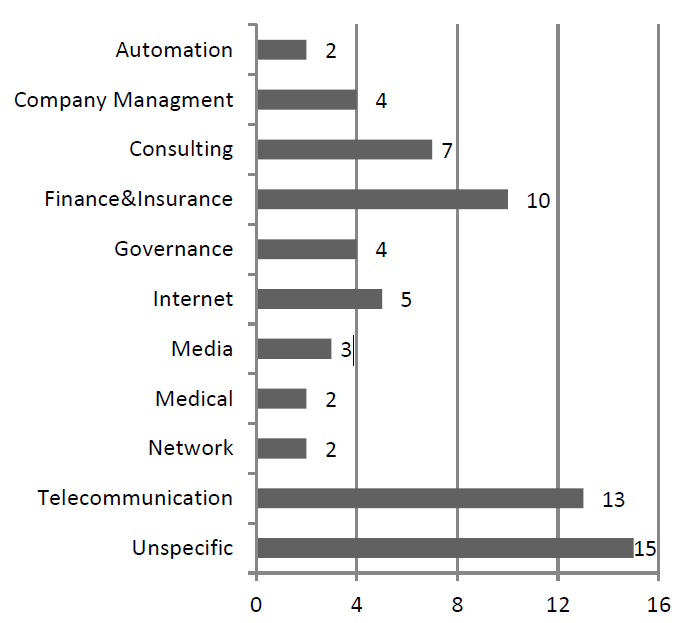
\includegraphics[width=90mm]{DieBold2014.png}
\caption{Agile distribution across domains \label{overflow}}
\end{figure}

Note the low occurrence of agile in the automation and medical industries. But problematic also is getting to a clear definition of what exactly agile software development entails. If the difference can only be regarded as iterative vs. incremental development practices, then agile methods have been in development since the 1970’s \cite{Larman_2003}. The latest iteration and most popular form of agile methods takes the shape of SCRUM, a process which specifies short development sprints of roughly two weeks in which certain developmental goals are specified and the team attempts to satisfy these goals. \cite{Cardozo_2010} did a literature review and found SCRUM did to lead to productivity improvements, but did not investigate if organisational make-up or the industry the company operates in have any effect. Also these findings are still very recent, and more in depth analysis is required.   

A couple of case studies have been performed on implementing agile methodologies in regulated industries. \cite{Fitzgerald_2013} found tension points when implementing a SCRUM process in a case study where the company and product had to comply with several FDA, ISO, IEC and ISPE regulations. These tension points were in quality assurance, safety and security, effectiveness, traceability, verification and validation. But even so it was found that agile can be suitable and even bring about improvements to regulated industry if tailored correctly. 

\cite{Shenvi_2014} also investigated if improvements can be made in the development of medical equipment when employing techniques from six sigma and agile, while complying with regulatory standards. A theoretical model was developed, and employed as a case study, resulting in improvements in productivity and a decrease in defects in the final product in the period the model was used between 2010 and 2013. It is unknown if wider applicability of the model exists for other industries with other certification requirements. 

\cite{Hrgarek_2012} pointed to further difficulties companies face in the medical device manufacturing industry when trying to employ agile methods while staying compliant with regulations. It is unclear if the case study was successful in employing agile methods into the development process.

\cite{Glas_2009} investigated a case in the application of agile methods in a aviation manufacturing setting, and identified open tool platforms and open design to be beneficial. The paper also mentioned regulatory difficulties as a problem for agile adoption, although this was not the focus of the study. 

In addition to agile methodologies such as SCRUM and Kanban etc, improvements have been made in developmental tools that aid in agile development. These tools include agile centric project management software, CI (Continuous integration), CD (Continuous deployment, Unit testing, TDD (Test driven development), BDD (Behaviour driven development), pair programming and others. 

\cite{Sfetsos_2010} did a literature survey and investigated which of the different agile tools does indeed provide improvements in product quality, and found TDD and pair programming to be beneficial. It should be noted that the study was performed in 2010, and a lot of improvements to agile has happened since then.

\cite{Causevic_2011} investigated uptake of TDD in industrial settings, and found the following limiting factors: increased development time, insufficient TDD experience/knowledge, lack of upfront design, domain and tool specific issues, lack of developer skill in writing test cases, insufficient adherence to TDD protocol, and legacy code. It is uncertain what is meant with an industrial setting, and if the companies involved was already engaged in other agile practices. 
 
\cite{Boehm_2003} shows that a balance between planned and agile methodologies can be found and formulates a strategy to arrive at such a balance. This paper is quite dated, especially given the velocity that agile is developing at, but represents a seminal work in blending agile and planned approaches from which several derivative works were produced. 

But even with the relatively slow uptake of agile in DO-178 projects, some work has been done on what high reliability agile would look like. The FDA (US Food and Drug Administration) released TIR45 \cite{AAMI_TIR45_2012}, which prescribes the application of agile software development practices for the development of safety critical medical devices seeking IEC 62304 certification. 

Furthermore Open-DO \cite{OPEN-DO_2010} is an initiative for the discussion of the application of agile methodologies to the DO-178C specification. Open-DO is a discussion platform and facilitated a conference in 2010 in France.     

\section{Survey on agile uptake in DO-178 projects}
For the purposes of this study survey responses were collected to answer the following questions about the current state of the DO-178 certified software industry:
\begin{enumerate}[A.]
\item Is there a case for agile development within the DO-178 %environment?
\item Is agile methods already being used within DO-178?
\item To get a benchmark to measure if agile methods improve DO-178 %development? 
\end{enumerate} 

The survey was advertised on various DO-178 special interest groups and mailing lists, technical news aggregator sites as well emails sent to the authors personal contacts active with DO-178 development (This explains the high amount of South African respondents).
 
The survey was completed by 88 respondents, in various roles, with various team sizes and in various countries:
\begin{table}[t!]
\centering
\caption{Roles}
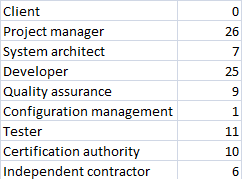
\includegraphics[width=60mm]{Roles.png}
\end{table}

\begin{figure}[t!]
\centering
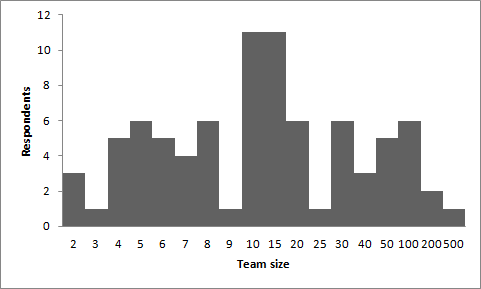
\includegraphics[width=90mm]{Teams.png}
\caption{Team size}
\end{figure}

\begin{table}[t!]
\centering
\caption{Countries}
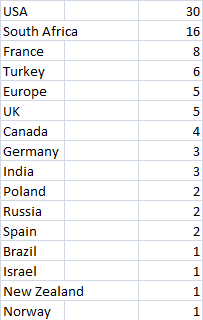
\includegraphics[width=50mm]{Countries.png}
\end{table}

Most respondents indicated they are still following the DO-178B specification and haven't switched over to the newer DO-178C specification which was released in January 2012.

\begin{table}[t!]
\centering
\caption{DO-178B and DO-178C use}
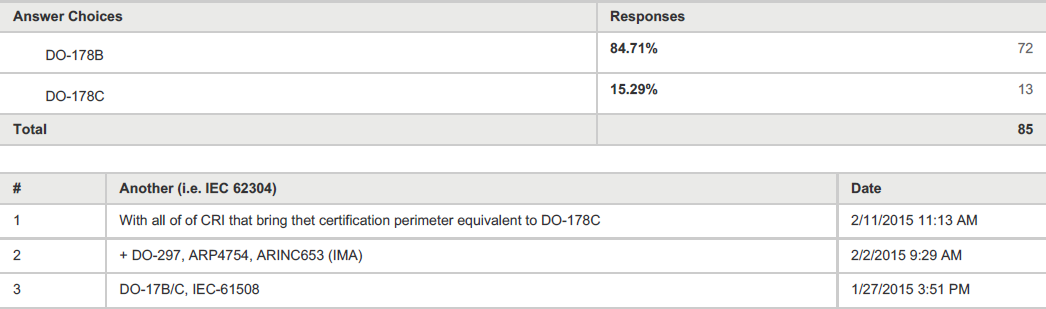
\includegraphics[width=90mm]{BvsC.png}
\end{table}

\subsection{A case for agile}
To determine if there is a case for the use of agile within DO-178, we looked at the current performance of DO-178 projects. This was done by asking the survey participants the following questions:

\begin{itemize}
	\item What was your last projects budget performance?
	\item What was your last project's delivery date performance?
	\item How many features was delivered according to the original specification?
	\item Was there any requests for additional features during the development? (Scope creep)
	\item Was there any requests for additional features after certification was complete? (Scope creep)
	\item In your opinion, does DO-178 increase the costs to a project? By how much?
\end{itemize}

\begin{table}[t!]
\centering
\caption{What was your last project's budget performance?}
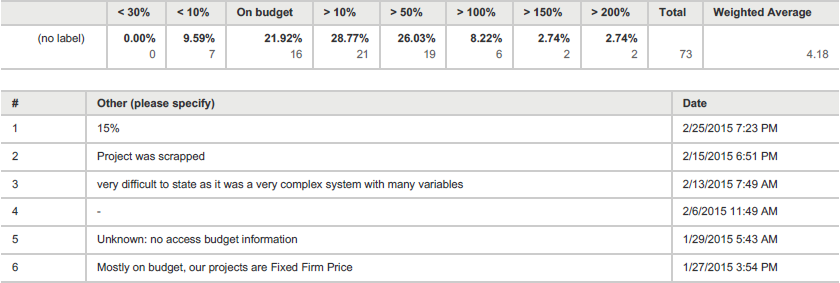
\includegraphics[width=90mm]{What_was_your_last_projects_budget_performance.png}
\end{table}

\begin{table}[t!]
\centering
\caption{What was your last project's delivery date performance?}
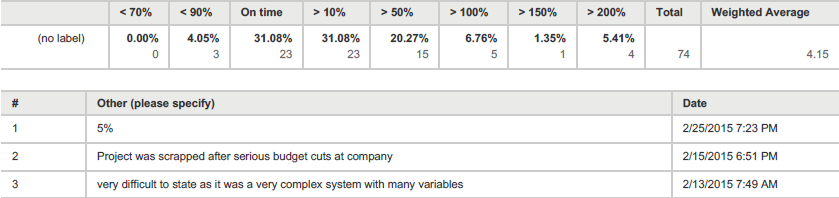
\includegraphics[width=90mm]{What_was_your_last_projects_delivery_date_performance.png}
\end{table}

\begin{table}[t!]
\centering
\caption{How many features was delivered according to the original specification?}
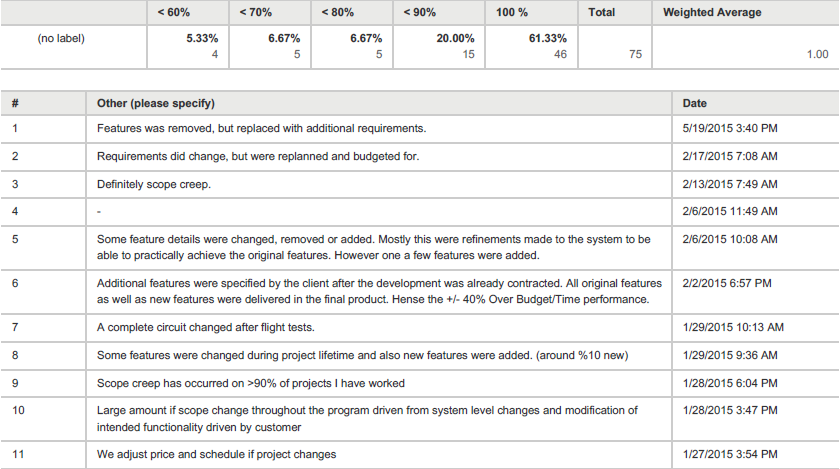
\includegraphics[width=90mm]{How_many_features_was_delivered_according_to_the_original_specification.png}
\end{table}

\begin{table}[t!]
\centering
\caption{Was there any requests for additional features during the development?}
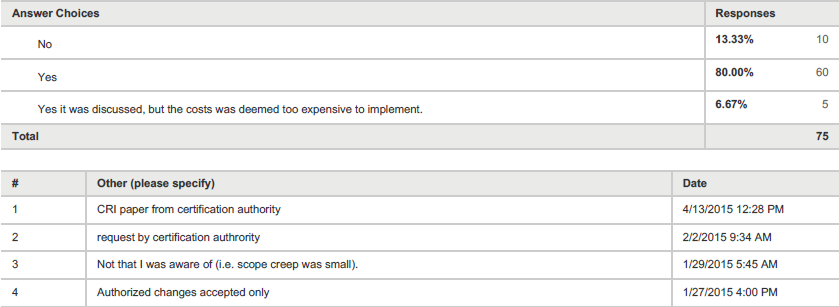
\includegraphics[width=90mm]{Was_there_any_requests_for_additional_features_during_the_development.png}
\end{table}

\begin{table}[t!]
\centering
\caption{Was there any requests for additional features after certification was complete?}
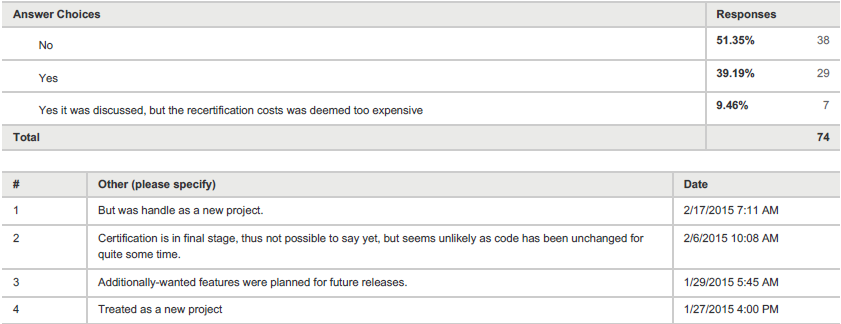
\includegraphics[width=90mm]{Was_there_any_requests_for_additional_features_after_certification_was_complete.png}
\end{table}

\begin{table}[t!]
\centering
\caption{In your opinion, does DO-178 increase the costs to a project?}
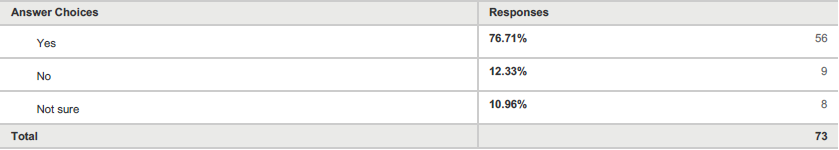
\includegraphics[width=90mm]{Does_increase_costs.png}
\end{table}

\begin{figure}[t!]
\centering 
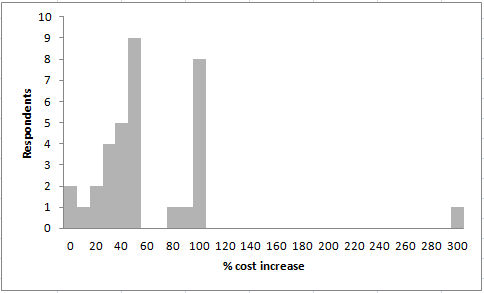
\includegraphics[width=90mm]{Cost_histogram.png}
\caption{By how much does costs increase?}
\end{figure}
%\FloatBarrier

\subsection{Is agile being used}
We also wanted to find out to which extent agile techniques were already being practiced in the industry. But not everybody in the industry agrees as to the same definition of what an agile development approach is. As such we asked the respondents if they were using a waterfall, rational unified process, kanban and scrum approach. We correlated this metric by asking respondents to confirm if they were using various developmental tools, some being agile orientated and some waterfall orientated. These responses were then correlated with the developmental approach responses, and measured for correlation. 

We also asked the respondents if they felt the development approach was helpful or not in their completion of their projects:

\begin{table}[t!]
\centering
\caption{Waterfall vs agile use}
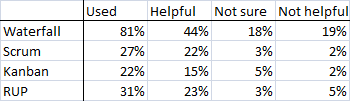
\includegraphics[width=60mm]{Agile_waterfall_uptake.png}
\end{table}

Note the percentages do not necessarily add up, as respondents may have filled in for multiple projects or multiple approaches may have been used within the same project (subcomponents for instance).    
 
\subsection{DO-178 benchmarks}
To measure the case study performance, the following benchmarks were gathered from the survey:
\begin{itemize}
	\item What is your \$ cost per line of code?
	\item What is your bugs per 1000 lines of code?
\end{itemize}
Off course these benchmarks presents difficulties of their own, such as inconsistent measuring...

\section{Conceptual model}

The following conceptual model were developed, taking inputs from TIR45 \cite{AAMI_TIR45_2012} and Open-DO \cite{OPEN-DO_2010}, but also taking general agile development principles, especially SCRUM and applying it to the required DO-178 outputs and objectives.

\begin{figure}[t!]
\centering 
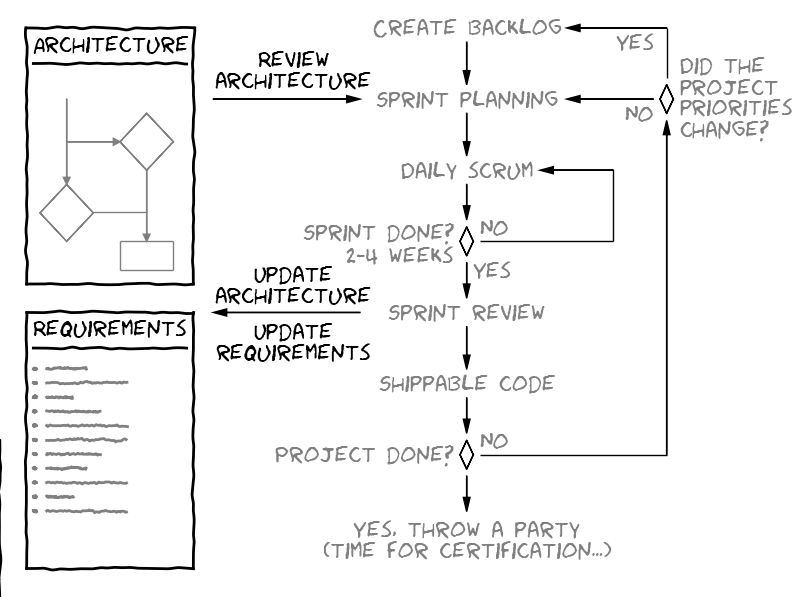
\includegraphics[width=90mm]{DO178_scrum.png}
\caption{Agile DO-178 framework}
\end{figure}

The conceptual model is focused on bringing continuous integration and continuous deployment to a DO-178 environment. The purposes is to reduce costs through automation of repeated processes. Since DO-178B is a software quality assurance standard, not a software development standard, it does not impose any restrictions or considerations on how software is to be developed. It does however require the following list of deliverables, with the requirements for each depending on the criticality level chosen:
\textbf{Organisational}
(These can be re-used across multiple projects, if the projects are similar enough off course):

\begin{itemize}
\item Software configuration management plan (SCM)
\item Software quality assurance plan (SQA)
\item Software requirements standards (SRS)
\item Software design standards (SDS)
\item Software code standards (SCS)
\item Software verification plan (SVP)
\end{itemize}

\textbf{At the start of a project - Specification phase:}

\begin{itemize}
\item Plan for software aspects of certification (PSAC)
\item Software development plan (SDP)
\item Software requirements data (SRD)
\item Design description (DD)
\end{itemize}

\textbf{During development - Implementation phase:}

\begin{itemize}
\item Source code
\item Object code
\item Software verification Cases and Procedures (SVCP)
\item Problem reports
\item Software Quality Assurance Records (SQA)
\item Software Configuration Management Records (SCMR)
\end{itemize}

\textbf{At the end of a project - Testing and verification phase:}

\begin{itemize}
\item Software Verification Results (SVR)
\item Software Life Cycle Environment Configuration Index (SECI)
\item Software Configuration Index (SCI)
\item Software Accomplishment Summary (SAS)
\end{itemize} 

The automated generation of some of these deliverables requires the development of infrastructure and tools that will facilitate a more agile way of working.

\begin{figure}[t!]
\centering 
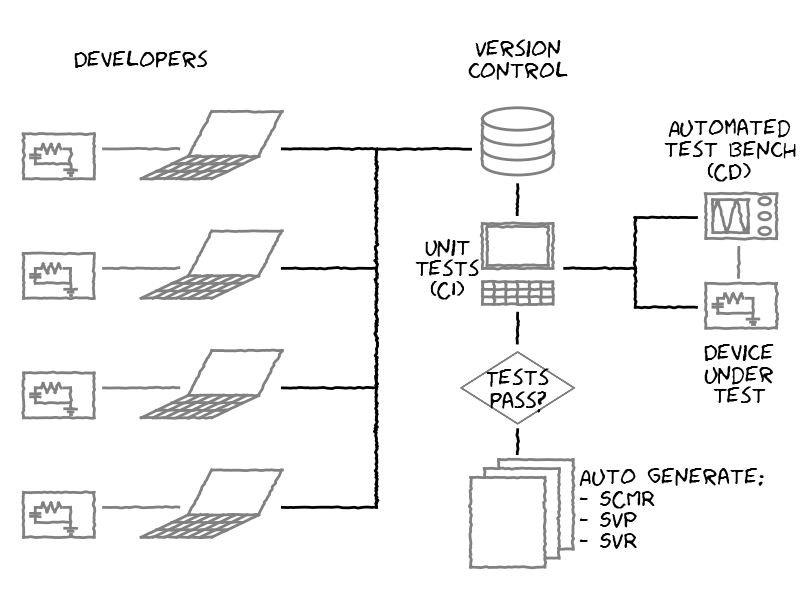
\includegraphics[width=90mm]{agile_setup.png}
\caption{Agile infrastructure}
\end{figure}

These automated generated outputs still has to comply with the DO-178 requirements on outputs as stipulated in the Annex A of the specification.

\section{Research design and methodology}

In order to test the effect that a more agile project management approach would have on a project requiring DO-178 certification, a case study was launched. In this case study two 3'rd year student teams developed and delivered a project according to exactly the same specification, with the one team running the agile workflow and the other a more traditional waterfall workflow.  

\begin{figure}[t!]
\centering 
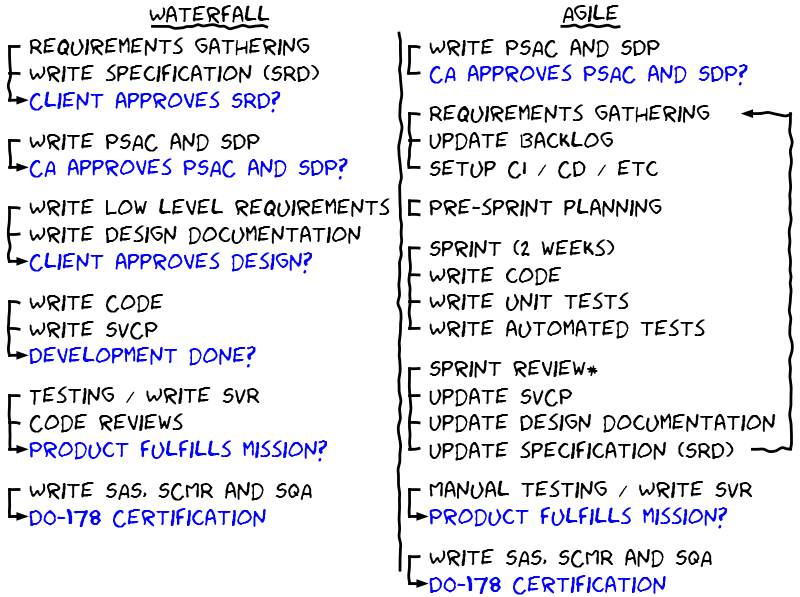
\includegraphics[width=90mm]{agileWaterfallTeamActivities.png}
\caption{Waterfall vs Agile comparison}
\end{figure}

The teams were tasked with developing group chat functionality for the Linphone open source project \cite{Linphone_2015}, and the final deliverable were measured for robustness of the solution, functionality delivered, maintainability, certification effort required, code bulk and the documentation bulk delivered.

Robustment were determined with independent functional testing of the solution, as well as the amount of unit tests and functional tests each team generated during development. 

Functionality delivered was a simple count against the original specification provided to each team.

Maintainability was determined by calculating the cyclomatic complexity of their code, as well as asking each team to give an estimate as to the effort required to develop additional functionality.

Certification effort still required were determined from external evaluation of each teams deliverables as measured against the DO-178 standard, and how close each team is to achieving a successful certification.

Code bulk is simply the count of lines of code delivered, documentation bulk is the word count of the documentation. Documentation also includes code comments.

Because the teams are not identical, in their size or their capability, a normalization task was given to each team. In this task, they were given exactly the same programming assignment to be completed in roughly half a day. The teams were measured on how long they took to complete the task and the quality of their final solution (how many bugs were still present). All case study metrics were then scaled against the results of this normalization exercise.

\section{Case study}

The 3rd year computer science students at the University of Pretoria has a year long subject where they complete a project as a team. This is the students first substantial project working as a team. These students are presented with a list of projects they are allowed to tender for. On this list was included two projects for this case study. Both projects listed exactly the same requirements, but it was stipulated that the one project will be run agile and the other waterfall. So some self selection of the students biased towards agile or waterfall workflows are present in the case study. For the tenders, six teams applied, three for each project. The two best applications were selected for this case study.

Interviews with Stacy and Freda still to take place middle September on how well the teams worked together, strengths and weaknesses of each team etc.

The agile team selected consists of six members and the waterfall team selected consists of five members. Team members from both teams have some experience with class projects they have completed, served as tutors in various but no large scale projects (multiple team members). Neither teams have experience with DO-178 certified software projects, and have only a theoretical understanding of agile and waterfall development practices.  

The teams submitted their tenders at the beginning of May 2015, and were notified of their successful application a week later. The first meeting between the teams and the client took place end of May after which the teams started their projects in earnest. The teams had about 6 months time from then on to complete the following list of identical requirements:
\begin{itemize}
\item Group chat (Invite additional members to a chat, all members receive chats)
\item Secure group chat (AES256)
\item Creation and deletion of groups
\item Voice record and send over IM
\item Rework the messaging user interface
	\begin{itemize}
	\item Spacing between words are terrible
	\item Make the text bigger
	\item Block indents required to better specify who said what
	\item Presence indication to show a remote user is typing
	\item User picture portraits
	\end{itemize}
\end{itemize}
Emphasis was placed with the student groups that the core requirement was the group chat functionality, then the encryption of the chats, and that all other requirements were of lesser importance. This was done to ensure both groups progress through the work similarly and that one group don't complete the easy work and the other the more difficult work items, which would make comparison difficult.  
 
\begin{figure}[t!]
\centering 
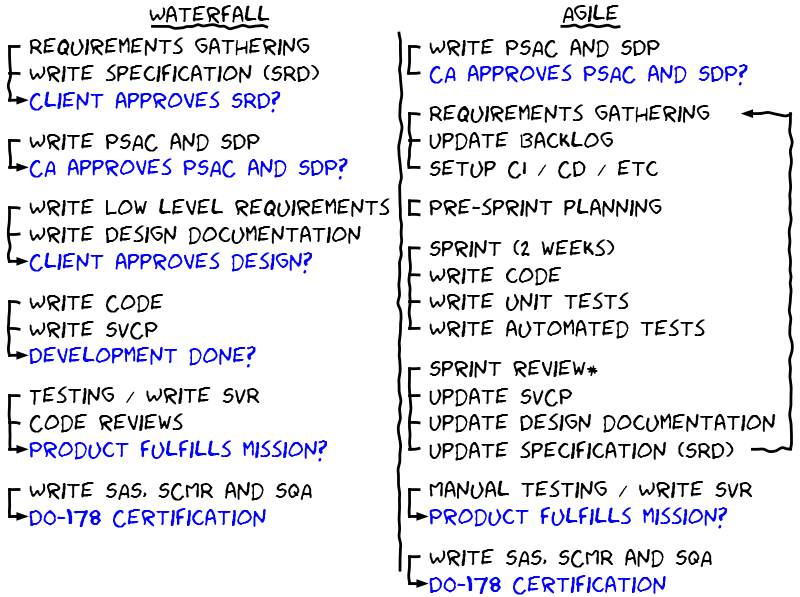
\includegraphics[width=90mm]{agileWaterfallTeamActivities.png}
\caption{Progress of the teams (TODO)}
\end{figure}


\section{Results}

Study is still running... will finish October / November.
Survey on students asking what they struggled with, how much time was spent on the project, estimation on adding features (robustness) etc still to be done (two weeks before final completion). 
Normalisation calibration still to take place middle October.

\section{Conclusion}
The conclusion goes here.




% conference papers do not normally have an appendix


% use section* for acknowledgement
\section*{Acknowledgment}


The authors would like to thank...

\begin{itemize}
\item Mr Kobus Steyn for his contribution on DO-178 considerations and best practices.
\item Ms Feziwe Mbatyoti for her external evaluation of the groups compliance to the DO-178 standard.
\item Ms Vreda Pieterse (lecturer) and Ms Stacy Omeleze (assistant lecturer) for their help with running the case study.
\\
\\
The following B.Sc Comp Sci students for participating in the study:
\item Patience Mtsweni
\item Lerato Molokomme
\item Tsepo Ntsaba
\item Mpedi Mello
\item Lutvyya Razak
\item Ephiphania Munava
\item Izak Blom
\item David Breetzke
\item Paul Engelke
\item Prenolan Govender
\item Jessica Lessev
\\ 
\end{itemize}
This study was completed as partial fulfilment of the requirements for the degree of: \\
\begin{center}Master of Engineering (MEM)\\
in the\\

GRADUATE SCHOOL OF TECHNOLOGY MANAGEMENT,\\
FACULTY OF ENGINEERING, BUILT ENVIRONMENT AND INFORMATION TECHNOLOGY,\\
UNIVERSITY OF PRETORIA
\end{center}

\bibliography{ref}
\bibliographystyle{IEEEtran}

% That's all folks!
\end{document}

